\documentclass{beamer}
\usetheme{Madrid}
\usecolortheme{default}
\usepackage{tikz}
\usepackage{amsmath}
\usepackage{booktabs}

% Title page information
\title{Causal Reasoning in the History of Science}
\subtitle{From Newton to Climate Change}
\author{Brendan Shea, PhD}
\date{Intro to Logic}

\begin{document}
	
	% Title slide
	\frame{\titlepage}
	
	% Slide 1: Causal Reasoning in Science: From Newton to Climate Change
	\begin{frame}{Causal Reasoning in Science: From Newton to Climate Change}
		\begin{itemize}
			\item Scientists face unique challenges when establishing \textbf{causal relationships} in natural phenomena that span vast scales of time and space.
			\item Unlike laboratory experiments, many scientific questions involve causes we cannot directly manipulate or control.
			\item Throughout history, major scientific breakthroughs required innovative methods to demonstrate causation without traditional experiments.
			\item Today we'll examine how scientists established causal claims that transformed our understanding of the universe.
		\end{itemize}
		
		\begin{block}{Our Journey Through Time}
			1687: Newton's Gravity → 1859: Darwin's Evolution → 1876: Germ Theory → 1950s: Smoking-Cancer Link → Today: Climate Change
		\end{block}
	\end{frame}
	
	% Slide 2: How Scientists Establish Causation: Beyond the Laboratory
	\begin{frame}{How Scientists Establish Causation: Beyond the Laboratory}
		\begin{itemize}
			\item Scientists use \textbf{converging evidence} from multiple sources when controlled experiments are impossible or impractical.
			\item Natural experiments, mathematical models, and careful observations can substitute for direct manipulation.
			\item \textbf{Predictive power} becomes crucial: if a causal theory correctly predicts new phenomena, it gains credibility.
			\item The scientific community requires extraordinary evidence for extraordinary causal claims that challenge existing beliefs.
		\end{itemize}
		
		\begin{example}[Types of Scientific Evidence]
			\begin{itemize}
				\item Observational data across time and space
				\item Natural experiments and comparative studies
				\item Mathematical models and simulations
				\item Mechanistic understanding of processes
			\end{itemize}
		\end{example}
	\end{frame}
	
	% Slide 3: The Challenge: Proving Causes in Complex Natural Systems
	\begin{frame}{The Challenge: Proving Causes in Complex Natural Systems}
		\begin{itemize}
			\item Natural systems involve \textbf{multiple interacting causes} that operate over different timescales and cannot be isolated.
			\item We cannot rerun Earth's history with different conditions or create control planets for comparison.
			\item \textbf{Temporal gaps} between causes and effects (like smoking and cancer) make causal inference difficult.
			\item Political, economic, and religious interests often resist scientific causal claims that threaten established systems.
		\end{itemize}
		
		\begin{alertblock}{The Fundamental Problem}
			How do we prove that invisible forces cause planetary motion, that random mutations cause new species, or that greenhouse gases cause global warming when we cannot perform controlled experiments?
		\end{alertblock}
	\end{frame}
	
	% Slide 4: Newton's Revolutionary Claim: Invisible Forces Cause Motion
	\begin{frame}{Newton's Revolutionary Claim: Invisible Forces Cause Motion}
		\begin{itemize}
			\item Newton proposed that an \textbf{invisible force} called gravity causes all objects with mass to attract each other.
			\item This claim was revolutionary because it suggested action without contact - objects affecting each other across empty space.
			\item Previous theories required physical contact or "vortices" of matter to explain motion and planetary orbits.
			\item Newton's mathematical approach allowed precise predictions without explaining \textit{how} gravity worked mechanistically.
		\end{itemize}
		
		\begin{block}{The Radical Idea}
			"Every particle in the universe attracts every other particle with a force proportional to the product of their masses and inversely proportional to the square of the distance between them."
			\[F = G\frac{m_1 m_2}{r^2}\]
		\end{block}
	\end{frame}
	
	% Slide 5: The Apple and the Moon: Unifying Terrestrial and Celestial Causation
	\begin{frame}{The Apple and the Moon: Unifying Terrestrial and Celestial Causation}
		\begin{itemize}
			\item Newton's insight was that the \textbf{same cause} explains both falling apples and orbiting moons.
			\item Before Newton, earthly and heavenly motion were thought to have completely different causes and follow different laws.
			\item By showing that moon's orbit and projectile motion follow the same mathematical principles, Newton unified physics.
			\item This \textbf{causal unification} was proven through calculation: the moon "falls" toward Earth at exactly the predicted rate.
		\end{itemize}
		
		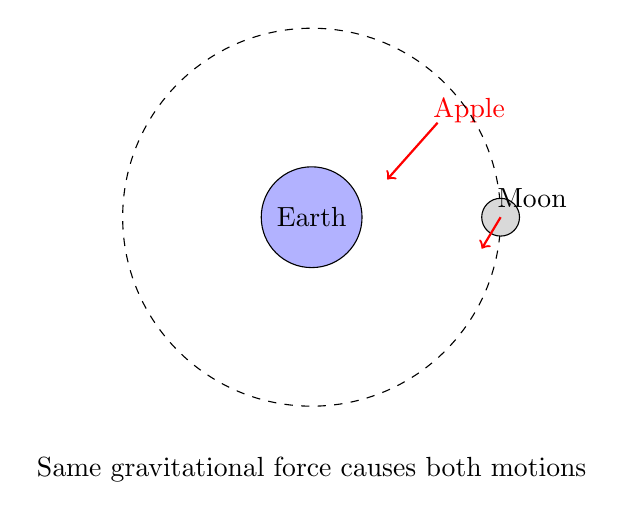
\begin{tikzpicture}[scale=0.8]
			% Earth
			\draw[fill=blue!30] (0,0) circle (0.8cm);
			\node at (0,0) {Earth};
			
			% Apple falling
			\draw[thick, red, ->] (2, 1.5) -- (1.2, 0.6);
			\node[red] at (2.5, 1.7) {Apple};
			
			% Moon orbiting
			\draw[dashed] (0,0) circle (3cm);
			\draw[fill=gray!30] (3,0) circle (0.3cm);
			\node at (3.5, 0.3) {Moon};
			\draw[thick, red, ->] (3, 0) -- (2.7, -0.5);
			
			% Label
			\node at (0, -4) {Same gravitational force causes both motions};
		\end{tikzpicture}
	\end{frame}
	
	% Slide 6: Mathematical Laws as Causal Explanations
	\begin{frame}{Mathematical Laws as Causal Explanations}
		\begin{itemize}
			\item Newton introduced the idea that \textbf{mathematical relationships} can serve as causal explanations in science.
			\item Rather than describing mechanisms, Newton's law precisely predicted how gravity's causal effects vary with mass and distance.
			\item Critics complained "hypotheses non fingo" (I frame no hypotheses) wasn't enough - they wanted to know \textit{why} gravity worked.
			\item Newton's success showed that mathematical descriptions of causal relationships could be scientifically valid without mechanical models.
		\end{itemize}
		
		\begin{example}[Causal Predictions from Math]
			\begin{itemize}
				\item Double the mass → Double the gravitational force
				\item Double the distance → Quarter the gravitational force  
				\item These precise relationships allowed testing causation through measurement
			\end{itemize}
		\end{example}
	\end{frame}
	
	% Slide 7: Prediction as Evidence: Halley's Comet Returns
	\begin{frame}{Prediction as Evidence: Halley's Comet Returns}
		\begin{itemize}
			\item Edmund Halley used Newton's gravitational theory to predict a comet would return in 1758 - decades after his own death.
			\item When the comet appeared exactly as predicted, it provided powerful evidence that gravity causes celestial motion.
			\item This \textbf{novel prediction} was more convincing than explaining already-known phenomena retroactively.
			\item The successful prediction demonstrated that Newton's causal theory could extend beyond observed data to future events.
		\end{itemize}
		
		\begin{alertblock}{The Power of Prediction}
			Successful predictions, especially of previously unknown phenomena, provide the strongest evidence for causal theories when experiments are impossible.
		\end{alertblock}
	\end{frame}
	
	% Slide 8: Action at a Distance: The Causal Controversy
	\begin{frame}{Action at a Distance: The Causal Controversy}
		\begin{itemize}
			\item Newton's gravity implied \textbf{action at a distance} - objects causing effects without touching, which many found absurd.
			\item Descartes and others insisted real causes required physical contact through "vortices" of swirling matter.
			\item Newton himself was uncomfortable with instantaneous action across empty space but couldn't explain the mechanism.
			\item The debate shows how causal claims that violate intuitions about "how causes work" face extra skepticism.
		\end{itemize}
		
		\begin{block}{Newton's Response}
			"I have not been able to discover the cause of those properties of gravity from phenomena, and I frame no hypotheses... It is enough that gravity does really exist, and acts according to the laws which we have explained."
		\end{block}
	\end{frame}
	
	% Slide 9: From Correlation to Causation: Planetary Orbits Explained
	\begin{frame}{From Correlation to Causation: Planetary Orbits Explained}
		\begin{itemize}
			\item Before Newton, astronomers had \textbf{correlations} - Kepler's laws described planetary motion patterns mathematically.
			\item Newton showed these patterns were \textbf{caused by} gravitational force, transforming description into explanation.
			\item Small deviations in orbits, previously dismissed as errors, were explained by gravitational pulls from other planets.
			\item This demonstrated how a true causal theory should explain both the regularities and the apparent exceptions.
		\end{itemize}
		
		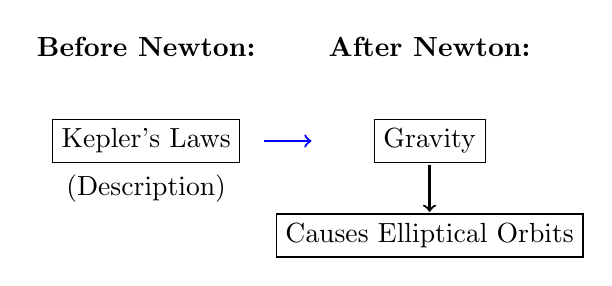
\begin{tikzpicture}[scale=0.6]
			% Before (correlation)
			\node at (-3, 2) {\textbf{Before Newton:}};
			\node[draw, rectangle] (kepler) at (-3, 0) {Kepler's Laws};
			\node at (-3, -1) {(Description)};
			
			% Arrow
			\draw[->, thick, blue] (-0.5, 0) -- (0.5, 0);
			
			% After (causation)
			\node at (3, 2) {\textbf{After Newton:}};
			\node[draw, rectangle] (gravity) at (3, 0) {Gravity};
			\draw[->, thick] (3, -0.5) -- (3, -1.5);
			\node[draw, rectangle] (orbits) at (3, -2) {Causes Elliptical Orbits};
		\end{tikzpicture}
	\end{frame}
	
	% Slide 10: Darwin's Causal Claim: Natural Selection Drives Species Change
	\begin{frame}{Darwin's Causal Claim: Natural Selection Drives Species Change}
		\begin{itemize}
			\item Darwin proposed that \textbf{natural selection} - differential survival and reproduction - causes species to evolve over time.
			\item This mechanism operates through variation, inheritance, and competition for limited resources in nature.
			\item Unlike Newton's instant forces, Darwin's cause operated over vast timescales invisible to human observation.
			\item The theory explained both the adaptation of organisms to their environments and the branching pattern of species relationships.
		\end{itemize}
		
		\begin{example}[The Causal Mechanism]
			\begin{enumerate}
				\item Individuals vary in traits
				\item Some traits aid survival/reproduction
				\item Beneficial traits are inherited
				\item Over generations, populations change
			\end{enumerate}
			Result: Natural selection causes evolution
		\end{example}
	\end{frame}
	
	% Slide 11: The Galápagos Finches: Natural Experiments in Evolution
	\begin{frame}{The Galápagos Finches: Natural Experiments in Evolution}
		\begin{itemize}
			\item The Galápagos Islands provided a \textbf{natural experiment} where similar finches evolved differently on different islands.
			\item Each island's unique environment (seeds, climate, competition) created different selection pressures.
			\item Darwin observed that beak shapes matched food sources - thick beaks where hard seeds dominated, thin where insects prevailed.
			\item This geographic variation suggested environmental conditions cause evolutionary changes through natural selection.
		\end{itemize}
		
		\begin{alertblock}{Natural Experiment Logic}
			If natural selection causes evolution, then:
			\begin{itemize}
				\item Similar species in different environments → Different adaptations
				\item Different species in similar environments → Convergent adaptations
			\end{itemize}
			Both patterns were observed!
		\end{alertblock}
	\end{frame}
	
	% Slide 12: Fossil Evidence: Causation Across Deep Time
	\begin{frame}{Fossil Evidence: Causation Across Deep Time}
		\begin{itemize}
			\item The \textbf{fossil record} provided historical evidence of evolution, showing species changing through geological time.
			\item Deeper (older) rock layers contained simpler organisms, while recent layers showed more complex forms.
			\item Transitional fossils like Archaeopteryx (reptile-bird) demonstrated intermediate forms predicted by evolutionary theory.
			\item This temporal sequence supported Darwin's claim that natural selection causes gradual transformation over millions of years.
		\end{itemize}
		
		\begin{block}{The Time Problem}
			\begin{center}
				Human lifetime: ~80 years\\
				Recorded history: ~5,000 years\\
				Species change: ~1,000,000+ years\\
				\vspace{0.2cm}
				How do we prove causation across unobservable timescales?
			\end{center}
		\end{block}
	\end{frame}
	
	% Slide 13: Artificial Selection: Controlled Experiments with Breeding
	\begin{frame}{Artificial Selection: Controlled Experiments with Breeding}
		\begin{itemize}
			\item Darwin used \textbf{artificial selection} in domesticated species as an experimental analog for natural selection.
			\item Pigeon breeders created dramatically different varieties by selecting which birds reproduced - proving selection causes change.
			\item In just dozens of generations, humans produced varieties as different as pugs and greyhounds from wolf ancestors.
			\item If human selection could cause such dramatic changes quickly, natural selection over millions of years could transform species.
		\end{itemize}
		
		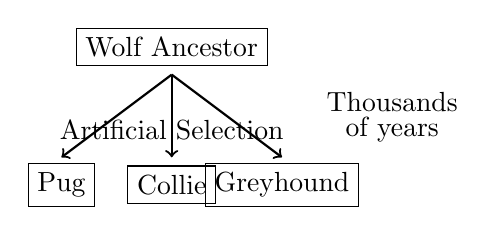
\begin{tikzpicture}[scale=0.7]
			% Original
			\node[draw, rectangle] (wolf) at (0, 0) {Wolf Ancestor};
			
			% Artificial selection
			\node at (0, -1.5) {Artificial Selection};
			\draw[->, thick] (0, -0.5) -- (-2, -2);
			\draw[->, thick] (0, -0.5) -- (0, -2);
			\draw[->, thick] (0, -0.5) -- (2, -2);
			
			% Results
			\node[draw, rectangle] (pug) at (-2, -2.5) {Pug};
			\node[draw, rectangle] (collie) at (0, -2.5) {Collie};
			\node[draw, rectangle] (grey) at (2, -2.5) {Greyhound};
			
			% Time scale
			\node at (4, -1) {Thousands};
			\node at (4, -1.5) {of years};
		\end{tikzpicture}
	\end{frame}
	
	% Slide 14: Biogeography: Why Isolation Causes Divergence
	\begin{frame}{Biogeography: Why Isolation Causes Divergence}
		\begin{itemize}
			\item \textbf{Biogeography} - the distribution of species across Earth - provided powerful evidence for evolution by natural selection.
			\item Islands contained unique species similar to, but distinct from, nearest mainland relatives, suggesting common ancestry.
			\item Geographic barriers (oceans, mountains) correlated with species boundaries, indicating isolation causes evolutionary divergence.
			\item The pattern made sense only if separation prevented interbreeding, allowing different selection pressures to cause different evolutionary paths.
		\end{itemize}
		
		\begin{example}[Biogeographic Evidence]
			\begin{tabular}{l|l}
				\textbf{Observation} & \textbf{Causal Inference} \\
				\hline
				Island species resemble mainland & Common ancestor \\
				But show unique adaptations & Local selection pressures \\
				More isolation = more difference & Time + selection = change \\
			\end{tabular}
		\end{example}
	\end{frame}
	
	% Slide 15: Modern DNA Evidence: Confirming Historical Causation
	\begin{frame}{Modern DNA Evidence: Confirming Historical Causation}
		\begin{itemize}
			\item \textbf{DNA evidence}, unavailable to Darwin, now provides molecular proof that natural selection causes evolutionary change.
			\item We can trace specific mutations and observe selection acting on them in real time in bacteria and viruses.
			\item Genetic similarities match the family tree predicted by fossils and biogeography, confirming common descent.
			\item DNA "molecular clocks" allow us to estimate when species diverged, validating the timescales Darwin proposed.
		\end{itemize}
		
		\begin{alertblock}{Converging Evidence}
			When multiple independent lines of evidence (fossils, biogeography, artificial selection, DNA) all support the same causal theory, scientists consider it confirmed beyond reasonable doubt.
		\end{alertblock}
	\end{frame}
	
	% Slide 16: Before Germs: Miasma Theory and Bad Air
	\begin{frame}{Before Germs: Miasma Theory and Bad Air}
		\begin{itemize}
			\item Before germ theory, the dominant \textbf{miasma theory} claimed diseases were caused by "bad air" from rotting matter.
			\item This theory seemed logical: diseases often occurred near swamps, sewage, and decay that produced foul odors.
			\item Correlation with smell led to causal inference - if places that smelled bad had more disease, smell must cause disease.
			\item The miasma theory led to some helpful practices (cleaning cities) but for the wrong causal reasons.
		\end{itemize}
		
		\begin{block}{The Miasma Mistake}
			\begin{center}
				Observed: Bad smells correlate with disease\\
				Inference: Bad air causes disease\\
				Reality: Microbes cause both bad smells AND disease\\
				\vspace{0.2cm}
				Classic case of confusing correlation with causation!
			\end{center}
		\end{block}
	\end{frame}
	
	% Slide 17: Pasteur's Experiments: Microbes Cause Fermentation and Disease
	\begin{frame}{Pasteur's Experiments: Microbes Cause Fermentation and Disease}
		\begin{itemize}
			\item Louis Pasteur demonstrated that \textbf{microorganisms} - not spontaneous generation or bad air - cause fermentation and decay.
			\item His swan-neck flask experiment proved that boiled broth stayed sterile unless exposed to airborne microbes.
			\item Pasteur then linked specific microbes to specific diseases, showing each disease had its own microbial cause.
			\item These controlled experiments revolutionized medicine by identifying the true \textbf{causal agents} of disease.
		\end{itemize}
		
		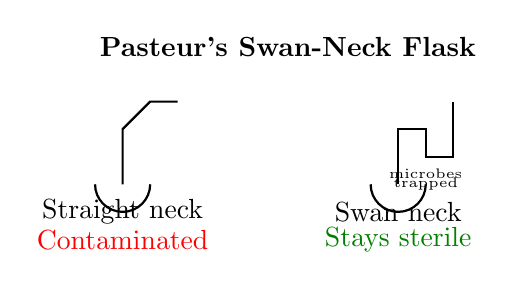
\begin{tikzpicture}[scale=0.7]
			% Swan neck flask experiment
			\node at (0, 2.5) {\textbf{Pasteur's Swan-Neck Flask}};
			
			% Flask 1 - straight neck
			\draw[thick] (-3, 0) -- (-3, 1) -- (-2.5, 1.5) -- (-2, 1.5);
			\draw[thick] (-3.5, 0) arc (180:360:0.5cm);
			\node at (-3, -0.5) {Straight neck};
			\node[red] at (-3, -1) {Contaminated};
			
			% Flask 2 - swan neck
			\draw[thick] (2, 0) -- (2, 1) -- (2.5, 1) -- (2.5, 0.5) -- (3, 0.5) -- (3, 1.5);
			\draw[thick] (1.5, 0) arc (180:360:0.5cm);
			\node at (2, -0.5) {Swan neck};
			\node[green!50!black] at (2, -1) {Stays sterile};
			
			% Microbes trapped
			\node at (2.5, 0.2) {\tiny microbes};
			\node at (2.5, 0) {\tiny trapped};
		\end{tikzpicture}
	\end{frame}
	
	% Slide 18: Koch's Postulates: Criteria for Microbial Causation
	\begin{frame}{Koch's Postulates: Criteria for Microbial Causation}
		\begin{itemize}
			\item Robert Koch developed four \textbf{postulates} - criteria to prove a specific microbe causes a specific disease.
			\item These postulates formalized how to establish causation when dealing with invisible agents and living hosts.
			\item Koch's systematic approach moved beyond correlation (microbe present in sick patients) to demonstration of causation.
			\item This framework became the gold standard for establishing microbial causation in infectious disease.
		\end{itemize}
		
		\begin{example}[Koch's Four Postulates]
			\begin{enumerate}
				\item Microbe must be found in all cases of the disease
				\item Microbe must be isolated and grown in pure culture
				\item Cultured microbe must cause disease when introduced to healthy host
				\item Microbe must be re-isolated from the new host
			\end{enumerate}
		\end{example}
	\end{frame}
	
	% Slide 19: Semmelweis and Handwashing: A Natural Experiment in Hospitals
	\begin{frame}{Semmelweis and Handwashing: A Natural Experiment in Hospitals}
		\begin{itemize}
			\item Ignaz Semmelweis noticed that wards staffed by doctors had higher maternal mortality than those staffed by midwives.
			\item He hypothesized that doctors performing autopsies carried \textbf{"cadaverous particles"} (germs) to patients.
			\item When handwashing with chlorine was implemented, mortality dropped from 18\% to 1\% - a natural experiment.
			\item Despite clear causal evidence, the medical establishment rejected his findings for decades, showing how paradigms resist change.
		\end{itemize}
		
		\begin{alertblock}{Resistance to Evidence}
			Semmelweis had data showing handwashing prevented deaths, but doctors rejected it because:
			\begin{itemize}
				\item It implied doctors were causing deaths
				\item Invisible germs seemed implausible
				\item It contradicted established miasma theory
			\end{itemize}
		\end{alertblock}
	\end{frame}
	
	% Slide 20: The Anthrax Breakthrough: Isolating a Specific Cause
	\begin{frame}{The Anthrax Breakthrough: Isolating a Specific Cause}
		\begin{itemize}
			\item Koch's work on \textbf{anthrax} in 1876 provided the first complete proof that a specific bacterium causes a specific disease.
			\item He isolated Bacillus anthracis from diseased animals, grew it in pure culture, and reproduced the disease in healthy animals.
			\item The anthrax lifecycle discovery explained puzzling observations like why certain fields remained "cursed" for decades.
			\item This success established the template for proving causation in infectious disease that we still use today.
		\end{itemize}
		
		\begin{block}{From Mystery to Mechanism}
			\begin{center}
				Before: "Cursed fields" where animals mysteriously died\\
				Koch's discovery: Anthrax spores survive in soil for years\\
				Result: Environmental persistence explained by bacterial biology\\
				\vspace{0.2cm}
				Understanding the causal agent explained the pattern!
			\end{center}
		\end{block}
	\end{frame}
	
	% Slide 21: Resistance and Acceptance: Why Causal Claims Face Skepticism
	\begin{frame}{Resistance and Acceptance: Why Causal Claims Face Skepticism}
		\begin{itemize}
			\item Germ theory faced fierce \textbf{resistance} from the medical establishment for decades despite mounting evidence.
			\item Accepting germs meant admitting that doctors had unknowingly caused deaths and that established treatments were useless.
			\item The theory required believing in invisible entities that seemed almost supernatural to many physicians.
			\item Acceptance came only after overwhelming evidence from multiple researchers and dramatic practical successes like antiseptic surgery.
		\end{itemize}
		
		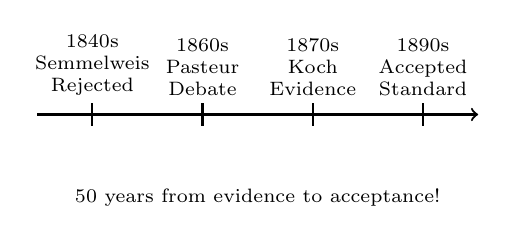
\begin{tikzpicture}[scale=0.7]
			\scriptsize
			% Timeline of acceptance
			\draw[thick, ->] (0,0) -- (8,0);
			
			% Events
			\draw[thick] (1, -0.2) -- (1, 0.2);
			\node[above, align=center] at (1, 0.2) {1840s\\Semmelweis\\Rejected};
			
			\draw[thick] (3, -0.2) -- (3, 0.2);
			\node[above, align=center] at (3, 0.2) {1860s\\Pasteur\\Debate};
			
			\draw[thick] (5, -0.2) -- (5, 0.2);
			\node[above, align=center] at (5, 0.2) {1870s\\Koch\\Evidence};
			
			\draw[thick] (7, -0.2) -- (7, 0.2);
			\node[above, align=center] at (7, 0.2) {1890s\\Accepted\\Standard};
			
			\node at (4, -1.5) {50 years from evidence to acceptance!};
		\end{tikzpicture}
	\end{frame}
	
	% Slide 22: The Epidemiological Challenge: When Experiments Are Unethical
	\begin{frame}{The Epidemiological Challenge: When Experiments Are Unethical}
		\begin{itemize}
			\item Proving that smoking causes cancer faced a unique challenge: we cannot ethically randomize people to smoke.
			\item Unlike infectious diseases, cancer develops over decades, making the causal link harder to establish.
			\item \textbf{Epidemiology} - studying disease patterns in populations - became the primary tool for establishing causation.
			\item Scientists had to develop new methods to prove causation without controlled experiments on humans.
		\end{itemize}
		
		\begin{example}[The Ethical Constraint]
			\textbf{Ideal experiment}: Randomly assign 10,000 people to smoke or not smoke for 30 years, measure cancer rates\\
			\textbf{Reality}: Completely unethical!\\
			\textbf{Solution}: Study people who choose to smoke vs. those who don't, controlling for confounders statistically
		\end{example}
	\end{frame}
	
	% Slide 23: Correlation Emerges: Early Statistical Links
	\begin{frame}{Correlation Emerges: Early Statistical Links}
		\begin{itemize}
			\item In the 1950s, researchers noticed strong \textbf{statistical correlations} between smoking rates and lung cancer deaths.
			\item Case-control studies found lung cancer patients were far more likely to be smokers than healthy controls.
			\item Cohort studies following thousands of people showed smokers developed lung cancer at 10-30 times the rate of non-smokers.
			\item The correlation was "dose-dependent" - heavy smokers had higher cancer rates than light smokers.
		\end{itemize}
		
		\begin{alertblock}{The Correlation Data (1950s)}
			\begin{center}
				Non-smokers: 10 lung cancer deaths per 100,000\\
				Light smokers: 50 lung cancer deaths per 100,000\\
				Heavy smokers: 300 lung cancer deaths per 100,000\\
				\vspace{0.2cm}
				But correlation isn't causation - what if smokers differ in other ways?
			\end{center}
		\end{alertblock}
	\end{frame}
	
	% Slide 24: The Tobacco Industry's Counter-Arguments: Confounders and Doubt
	\begin{frame}{The Tobacco Industry's Counter-Arguments: Confounders and Doubt}
		\begin{itemize}
			\item The tobacco industry exploited the correlation-causation distinction to manufacture \textbf{doubt} about the smoking-cancer link.
			\item They proposed alternative explanations: genetic predisposition, personality types, air pollution, or other lifestyle factors.
			\item Industry-funded scientists emphasized that without randomized experiments, causation couldn't be "proven" definitively.
			\item This strategy of "doubt is our product" delayed public health action for decades despite mounting evidence.
		\end{itemize}
		
		\begin{block}{Manufacturing Doubt}
			\scriptsize
			\textbf{Tobacco Industry Playbook:}
			\begin{itemize}
				\item "Correlation doesn't prove causation"
				\item Fund studies looking for other explanations
				\item Demand impossible standard of proof
				\item Emphasize any uncertainty in the science
			\end{itemize}
			Result: Public confusion despite scientific consensus
		\end{block}
	\end{frame}
	
	% Slide 25: Hill's Criteria: Nine Tests for Causation Without Experiments
	\begin{frame}{Hill's Criteria: Nine Tests for Causation Without Experiments}
		\begin{itemize}
			\item In 1965, Austin Bradford Hill proposed nine \textbf{criteria} for establishing causation from observational data (when no experiment is possible).
			\item Hill emphasized that no single criterion was necessary or sufficient - rather, the totality of evidence mattered.
		\end{itemize}
		
		\begin{example}[Hill's Nine Criteria]
			\scriptsize
			\begin{enumerate}
				\item \textbf{Strength}: How strong is the association?
				\item \textbf{Consistency}: Observed by different researchers?
				\item \textbf{Specificity}: Specific exposure, specific disease?
				\item \textbf{Temporality}: Exposure precedes disease?
				\item \textbf{Biological gradient}: Dose-response curve?
				\item \textbf{Plausibility}: Biologically plausible?
				\item \textbf{Coherence}: Fits with other knowledge?
				\item \textbf{Experiment}: Natural experiments exist?
				\item \textbf{Analogy}: Similar causes known?
			\end{enumerate}
		\end{example}
	\end{frame}
	
	% Slide 26: Converging Evidence: Animal Studies, Mechanisms, and Dose-Response
	\begin{frame}{Converging Evidence: Animal Studies, Mechanisms, and Dose-Response}
		\begin{itemize}
			\item \textbf{Animal experiments} showed that tobacco tar painted on mice skin caused tumors, providing experimental evidence.
			\item Scientists identified carcinogens in tobacco smoke and traced the biological mechanisms of DNA damage.
			\item The \textbf{dose-response relationship} - more smoking meant more cancer risk - strongly suggested causation.
			\item Multiple independent lines of evidence all pointed to the same conclusion: smoking causes cancer.
		\end{itemize}
		
		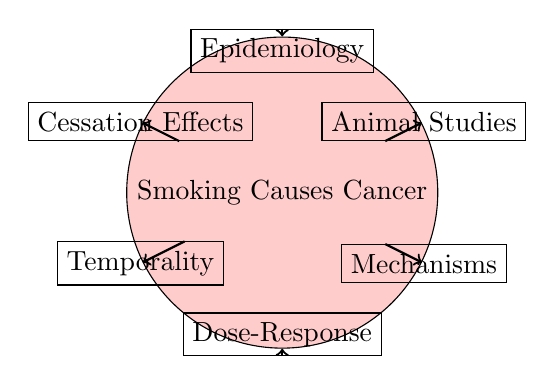
\begin{tikzpicture}[scale=0.6]
			% Center node
			\node[draw, circle, fill=red!20] (center) at (0,0) {Smoking Causes Cancer};
			
			% Evidence nodes
			\node[draw, rectangle] (epi) at (0, 3) {Epidemiology};
			\node[draw, rectangle] (animal) at (3, 1.5) {Animal Studies};
			\node[draw, rectangle] (mech) at (3, -1.5) {Mechanisms};
			\node[draw, rectangle] (dose) at (0, -3) {Dose-Response};
			\node[draw, rectangle] (time) at (-3, -1.5) {Temporality};
			\node[draw, rectangle] (cess) at (-3, 1.5) {Cessation Effects};
			
			% Arrows
			\draw[->, thick] (epi) -- (center);
			\draw[->, thick] (animal) -- (center);
			\draw[->, thick] (mech) -- (center);
			\draw[->, thick] (dose) -- (center);
			\draw[->, thick] (time) -- (center);
			\draw[->, thick] (cess) -- (center);
		\end{tikzpicture}
	\end{frame}
	
	% Slide 27: Policy Implications: From Causal Knowledge to Public Health
	\begin{frame}{Policy Implications: From Causal Knowledge to Public Health}
		\begin{itemize}
			\item The U.S. Surgeon General's 1964 report officially declared smoking a \textbf{cause} of lung cancer, not just a correlation.
			\item This causal determination justified public health interventions: warning labels, advertising bans, and smoke-free spaces.
			\item Smoking rates dropped from 42\% (1965) to 14\% (2019) in the U.S., preventing millions of deaths.
			\item The smoking case established precedents for how epidemiological evidence can support causal claims and policy action.
		\end{itemize}
		
		\begin{alertblock}{The Power of Causal Knowledge}
			\begin{center}
				1950s: "Smoking is correlated with cancer" → Limited action\\
				1964: "Smoking CAUSES cancer" → Public health revolution\\
				\vspace{0.2cm}
				Establishing causation, not just correlation, enables effective intervention
			\end{center}
		\end{alertblock}
	\end{frame}
	% Slide 28: The Greenhouse Effect: From 19th Century Theory to Modern Crisis
	\begin{frame}{The Greenhouse Effect: From 19th Century Theory to Modern Crisis}
		\begin{itemize}
			\item In 1859, John Tyndall discovered that \textbf{CO$_2$ and water vapor} trap heat, proposing the greenhouse effect mechanism.
			\item Svante Arrhenius (1896) calculated that doubling atmospheric CO$_2$ would cause 5-6°C warming - remarkably close to modern estimates.
			\item These early scientists identified the causal mechanism decades before any warming was observable.
			\item The theoretical foundation preceded the evidence, showing how understanding mechanisms can predict future causation.
		\end{itemize}
		
		\begin{block}{The Causal Chain}
			\begin{center}
				Burning fossil fuels → Increases atmospheric CO$_2$ →\\
				CO$_2$ traps infrared radiation → Earth's temperature rises →\\
				Climate patterns change globally\\
				\vspace{0.2cm}
				Mechanism understood 160+ years ago!
			\end{center}
		\end{block}
	\end{frame}
	
	% Slide 29: Multiple Lines of Evidence: Temperature Records and Ice Cores
	\begin{frame}{Multiple Lines of Evidence: Temperature Records and Ice Cores}
		\begin{itemize}
			\item Global temperature records show approximately 1.1°C warming since pre-industrial times, matching theoretical predictions.
			\item \textbf{Ice cores} provide 800,000 years of climate history, showing CO$_2$ and temperature move together throughout Earth's history.
			\item Current CO$_2$ levels (420+ ppm) are the highest in over 3 million years, far exceeding natural variations.
			\item Multiple independent datasets (land, ocean, satellite, balloon) all show consistent warming patterns.
		\end{itemize}
		
		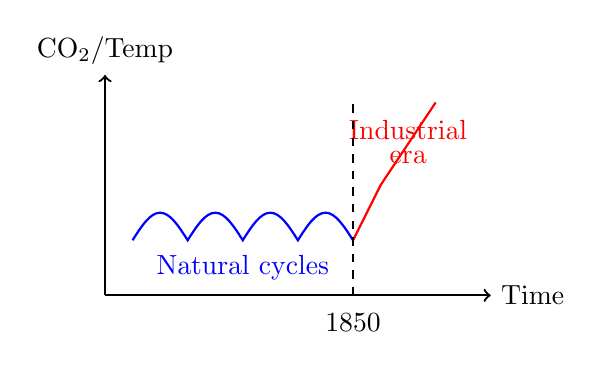
\begin{tikzpicture}[scale=0.7]
			% Graph axes
			\draw[thick, ->] (0,0) -- (7,0) node[right] {Time};
			\draw[thick, ->] (0,0) -- (0,4) node[above] {CO$_2$/Temp};
			
			% Natural variation
			\draw[blue, thick] (0.5,1) sin (1,1.5) cos (1.5,1) sin (2,1.5) cos (2.5,1) sin (3,1.5) cos (3.5,1) sin (4,1.5) cos (4.5,1);
			\node[blue] at (2.5, 0.5) {Natural cycles};
			
			% Industrial spike
			\draw[red, thick] (4.5,1) -- (5,2) -- (6,3.5);
			\node[red] at (5.5, 3) {Industrial};
			\node[red] at (5.5, 2.5) {era};
			
			% Label
			\draw[dashed] (4.5, 0) -- (4.5, 3.5);
			\node at (4.5, -0.5) {1850};
		\end{tikzpicture}
	\end{frame}
	
	% Slide 30: Natural Experiments: Volcanic Eruptions as Climate Tests
	\begin{frame}{Natural Experiments: Volcanic Eruptions as Climate Tests}
		\begin{itemize}
			\item Major \textbf{volcanic eruptions} provide natural experiments by injecting aerosols that temporarily cool the planet.
			\item The 1991 Mount Pinatubo eruption caused ~0.5°C global cooling for 2-3 years, exactly as climate models predicted.
			\item These events test our understanding of climate causation - if models correctly predict volcanic cooling, they likely capture warming mechanisms too.
			\item The temporary cooling followed by resumed warming strengthens evidence that CO$_{2}$, not natural factors, drives long-term trends.
		\end{itemize}
		
		\begin{example}[Pinatubo as Natural Experiment]
			\begin{itemize}
				\item Prediction (1991): Models forecast 0.5°C cooling
				\item Observation (1992-93): 0.5°C cooling occurred
				\item Result: Successful prediction validates climate models
				\item Implication: Same models show CO$_{2}$ causes warming
			\end{itemize}
		\end{example}
	\end{frame}
	
	% Slide 31: Computer Models: Simulating Causal Mechanisms
	\begin{frame}{Computer Models: Simulating Causal Mechanisms}
		\begin{itemize}
			\item \textbf{Climate models} integrate known physical laws to simulate Earth's climate system and test causal hypotheses.
			\item Models can run "experiments" impossible in reality: Earth with/without human emissions, doubled CO$_{2}$, removed ice caps.
			\item Only models including human CO$_{2}$ emissions reproduce observed 20th-century warming - natural factors alone cannot.
			\item Multiple independent modeling groups worldwide reach the same conclusions, providing consistency across approaches.
		\end{itemize}
		
		\begin{alertblock}{The Fingerprint Test}
			Models run with only natural causes (solar, volcanic) = No warming trend\\
			Models run with only human causes (CO$_{2}$, aerosols) = Matches observations\\
			Models with both natural + human causes = Best match to reality\\
			\vspace{0.2cm}
			This "fingerprinting" identifies human causation
		\end{alertblock}
	\end{frame}
	
	% Slide 32: The Attribution Problem: Separating Human from Natural Causes
	\begin{frame}{The Attribution Problem: Separating Human from Natural Causes}
		\begin{itemize}
			\item \textbf{Attribution science} works to separate human-caused climate change from natural variability like El Niño and solar cycles.
			\item Scientists use "detection and attribution" studies comparing observed patterns to those expected from different causes.
			\item Human causation creates distinct "fingerprints": warming troposphere but cooling stratosphere, Arctic amplification, changing seasons.
			\item Natural causes alone cannot explain observed changes - only human factors produce the right pattern and magnitude.
		\end{itemize}
		
		\begin{block}{Causal Fingerprints}
			\begin{tabular}{l|l}
				\textbf{Observation} & \textbf{Indicates} \\
				\hline
				Stratosphere cooling & Greenhouse gases (not solar) \\
				Arctic warms fastest & Ice-albedo feedback \\
				Nights warm more than days & Heat trapping \\
				Ocean warming at depth & Long-term forcing \\
			\end{tabular}
		\end{block}
	\end{frame}
	
	% Slide 33: Scientific Consensus: When Multiple Methods Confirm Causation
	\begin{frame}{Scientific Consensus: When Multiple Methods Confirm Causation}
		\begin{itemize}
			\item Over 99\% of climate scientists agree that humans are causing current global warming - extraordinary consensus.
			\item This agreement arose from \textbf{convergent evidence}: physics, observations, experiments, and models all point to human causation.
			\item Like evolution and germ theory before it, climate science faced initial skepticism but evidence accumulated overwhelmingly.
			\item Scientific consensus doesn't determine truth, but when multiple independent methods agree, confidence in causation increases.
		\end{itemize}
		
		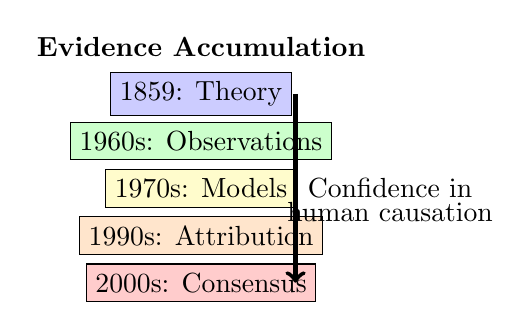
\begin{tikzpicture}[scale=0.6]
			% Timeline of evidence accumulation
			\node at (0, 3) {\textbf{Evidence Accumulation}};
			
			% Boxes for different types
			\node[draw, rectangle, fill=blue!20] (theory) at (0, 2) {1859: Theory};
			\node[draw, rectangle, fill=green!20] (obs) at (0, 1) {1960s: Observations};
			\node[draw, rectangle, fill=yellow!20] (models) at (0, 0) {1970s: Models};
			\node[draw, rectangle, fill=orange!20] (attr) at (0, -1) {1990s: Attribution};
			\node[draw, rectangle, fill=red!20] (cons) at (0, -2) {2000s: Consensus};
			
			% Arrow showing progression
			\draw[->, ultra thick] (2, 2) -- (2, -2);
			\node at (4, 0) {Confidence in};
			\node at (4, -0.5) {human causation};
		\end{tikzpicture}
	\end{frame}
	
	% Slide 34: Common Patterns: How Science Establishes Causation
	\begin{frame}{Common Patterns: How Science Establishes Causation}
		\begin{itemize}
			\item Across all our cases, scientists used \textbf{multiple independent lines of evidence} to establish causation without perfect experiments.
			\item \textbf{Predictive success} proved crucial: Halley's comet, vaccine effectiveness, cancer rates, volcanic cooling all validated theories.
			\item Understanding \textbf{mechanisms} strengthened causal claims: gravity equations, natural selection, germs, carcinogens, greenhouse physics.
			\item Natural experiments and comparative studies substituted for controlled experiments when manipulation was impossible or unethical.
		\end{itemize}
		
		\begin{example}[Universal Strategies]
			\begin{itemize}
				\item Theory predicts → Observation confirms
				\item Multiple methods → Same conclusion
				\item Dose-response → Strengthens causation
				\item Mechanisms explain → Patterns observed
				\item Natural variation → Tests hypotheses
			\end{itemize}
		\end{example}
	\end{frame}
	
	% Slide 35: The Role of Time: Why Accepting Causal Claims Takes Decades
	\begin{frame}{The Role of Time: Why Accepting Causal Claims Takes Decades}
		\begin{itemize}
			\item Major causal claims in science typically take \textbf{30-50 years} from initial proposal to general acceptance.
			\item This delay reflects both healthy skepticism and resistance from those whose interests are threatened by new knowledge.
			\item Time allows evidence to accumulate, predictions to be tested, and alternative explanations to be ruled out.
			\item Each case study shows a similar pattern: early pioneers face rejection, evidence accumulates, and eventually paradigms shift.
		\end{itemize}
		
		\begin{alertblock}{The Pattern of Acceptance}
			\begin{center}
				Initial claim → Fierce resistance → Evidence accumulates →\\
				Predictions confirmed → Alternative explanations fail →\\
				New generation of scientists → Paradigm shift →\\
				"How could anyone have doubted this?"
			\end{center}
		\end{alertblock}
	\end{frame}
	
	% Slide 36: Lessons for Today: Evaluating Scientific Causal Claims
	\begin{frame}{Lessons for Today: Evaluating Scientific Causal Claims}
		\begin{itemize}
			\item When evaluating scientific causal claims, look for \textbf{convergent evidence} from multiple independent sources and methods.
			\item Be suspicious of demands for impossible proof or those who emphasize uncertainty without acknowledging the weight of evidence.
			\item Recognize that those with financial or ideological stakes often manufacture doubt about inconvenient causal relationships.
			\item Remember that science's strength lies not in any single study but in the accumulation and integration of evidence over time.
		\end{itemize}
		
		\begin{block}{Your Scientific Reasoning Toolkit}
			\begin{center}
				$\checkmark$ Does the proposed mechanism make sense?\\
				$\checkmark$ Do multiple lines of evidence converge?\\
				$\checkmark$ Are predictions being confirmed?\\
				$\checkmark$ Who benefits from denial?\\
				$\checkmark$ What do experts in the field conclude?\\
				$\checkmark$ How long has evidence been accumulating?
			\end{center}
		\end{block}
	\end{frame}
\end{document}